% !TeX spellcheck = en_US
\documentclass[10pt,a4paper,titlepage]{article}
\usepackage[latin1]{inputenc}
\usepackage{amsmath}
\usepackage{amsfonts}
\usepackage{amssymb}
\usepackage{makeidx}
\usepackage{graphicx}
\usepackage[left=2.00cm, right=2.00cm, top=2.00cm, bottom=2.00cm]{geometry}
\usepackage{tikz}
\usepackage{tikz-uml}
\usetikzlibrary{patterns}%for tikz https://tex.stackexchange.com/questions/54464/hatch-a-rectangle-in-tikz

%Makes index browsable in pdf viewers and shows index in sidebar
\usepackage[bookmarks]{hyperref}
\author{Mikail Gedik}
\title{Thesis Paper}
\begin{document}
	\pagenumbering{roman}
	\maketitle
	\tableofcontents
	\listoffigures
	\clearpage
	\pagenumbering{arabic}
	\section{Abstract}
	This paper tackles the calculation of a few selected fractals and shines light on the core aspects I have implemented and furthermore optimized to use all the resources provided by the computer. My journey begins at a single threaded Java program and ends in a multi threaded C application able to make use graphics cards. Additionally, I will make an easy-to use yet powerful UI, which will enable even tech-unfamiliar people to use my software.
	\subsection{Program Capabilities \& Expectations}
	Here I will be listing all capabilities my program should have, from easiest to hardest.
	\subsection{General}
	\subsubsection{Operating System Independence}
	As a Linux user, I am heavily outnumbered by Windows and Mac users. Because of this, my software has to run on the other platforms, or else very few people will be able to test or run my program. Due to me beginning the project in Java, this will only become an issue when switching to C++. I will be using the Vulkan API to use video cards, which is also platform independent and shouldn't cause any issues.
	\subsection{Backend}
	\subsubsection{Basic Java Single Threaded Mandelbrot Set Calculation}
	The first goal is to make a simple Java program, which will calculate the Mandelbrot set and output the result into a file. It is not yet intended to be structurally divided and good as shown in figure \ref{fig:program_structure} (Page \pageref{fig:program_structure}), but more closely together as there are yet not enough parts to separate the code.\\
	Next up would be the implementation of the settings using a simple database like a list.
	\subsubsection{Basic Java Single Threaded Mandelbrot Set Calculation}
	\subsection{Windowed Frontend}
	\subsection{Other Known Programs}
	
	
	\section{Program Structure}
	
	%\begin{tikzpicture}
	%	\begin{umlpackage}[x=0,y=0]{package-name}
	%	\end{umlpackage}
	%\end{tikzpicture}
	
	My program is separated in two halves, the front- and backend. While the latter is autonomous, the former is dependent on the backend, as it must know its interface, which is the connecting bridge between them. The front-end can request or order a command through a command string or an integer, i. e. a character sequence or a number. The backend answer these with a command result, which may also be an image.\\
	Because the backend is detached from the front-end, I may also develop multiple front-ends for different needs. The front-end in the diagram below shows a possible version of window-oriented front-end, which is relatively modern and user-friendly, but for example useless in a command line environment. Thus I see the need to develop different front-ends.
	
		\begin{figure}
			\centering
			\caption{Program structure}
			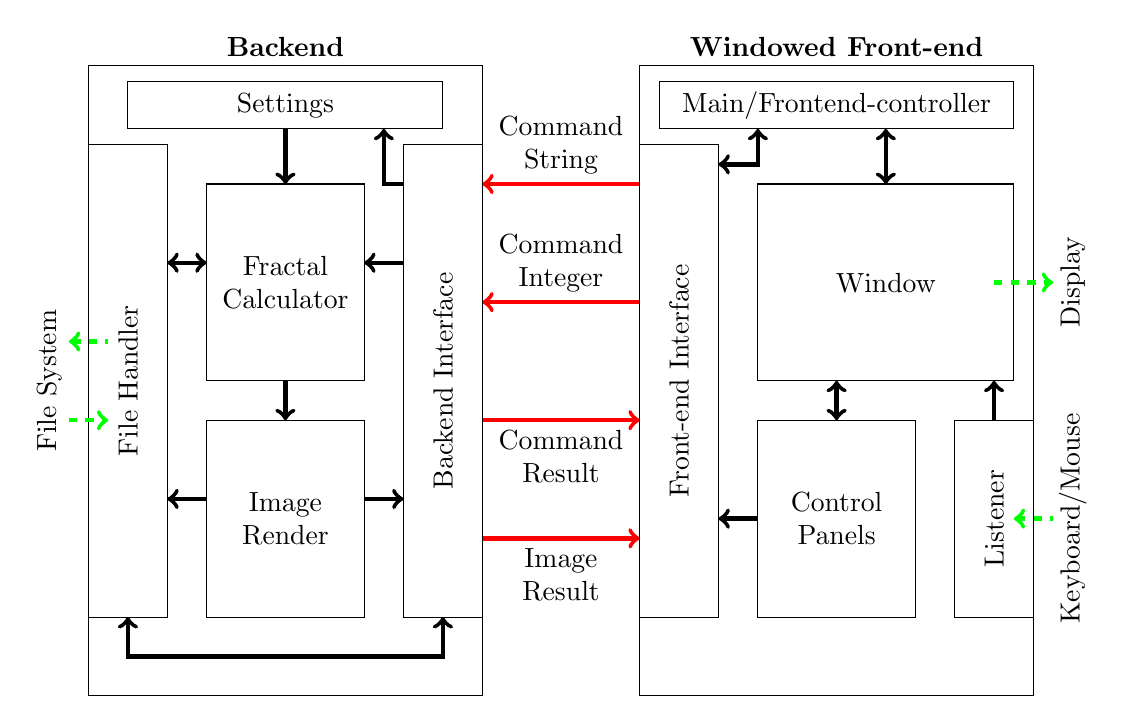
\begin{tikzpicture}
			%Front/Backend-connection
			\draw[red, ultra thick, <-] (5,6.5) -- (7,6.5);
			\node[above, align=center] at (6,6.5) {Command\\String};
			
			\draw[red, ultra thick, <-] (5,5) -- (7,5);
			\node[above, align=center] at (6,5) {Command\\Integer};
			
			\draw[red, ultra thick, ->] (5,3.5) -- (7,3.5);
			\node[below, align=center] at (6,3.5) {Command\\Result};
			
			\draw[red, ultra thick, ->] (5,2) -- (7,2);
			\node[below, align=center] at (6,2) {Image\\Result};
			
			%Backend
			\draw (0,0) rectangle (5,8);
			\node[above] at (2.5, 8) {\textbf{Backend}};
			
			%Interface
			\draw (4,1) rectangle (5, 7);
			\node[rotate = 90] at(4.5, 4) {Backend Interface};
			
			%Settings
			\draw (.5,7.2) rectangle (4.5, 7.8);
			\node at (2.5, 7.5) {Settings};
			
			%Fractal calculator
			\draw (1.5,4) rectangle (3.5, 6.5);
			\node[align=center] at (2.5, 5.25) {Fractal\\Calculator};
			
			%Image render
			\draw (1.5,1) rectangle (3.5, 3.5);
			\node[align=center] at (2.5, 2.25) {Image\\Render};
			
			%File handling
			\draw (0,1) rectangle (1, 7);
			\node[rotate = 90] at(.5, 4) {File Handler};
			
			%Arrows
			%Settings-Frac
			\draw[ultra thick, ->] (2.5, 7.2) -- (2.5, 6.5);
			%Int-Frac
			\draw[ultra thick, <-] (3.5, 5.5) -- (4, 5.5);
			%Frac-Image
			\draw[ultra thick, ->]  (2.5, 4) -- (2.5, 3.5);
			%Img-Int
			\draw[ultra thick, ->]  (3.5, 2.5) -- (4, 2.5);
			%Frac-File
			\draw[ultra thick, <->] (1.5, 5.5) -- (1, 5.5);
			%Image-File
			\draw[ultra thick, ->] (1.5, 2.5) -- (1, 2.5);
			%Settings-Int
			\draw[ultra thick, ->] (4, 6.5) -- (3.75, 6.5) -- (3.75, 7.2); 
			%Int-File
			\draw[ultra thick, <->] (4.5, 1) -- (4.5,.5) -- (.5,.5) -- (.5, 1);
			
			%File system
			\draw[green, ultra thick, dashed, ->] (-.25, 3.5) -- (.25, 3.5);
			\draw[green, ultra thick, dashed, <-] (-.25, 4.5) -- (.25, 4.5);
			\node[rotate = 90] at (-.5, 4) {File System};
			
			%Frontend
			\draw (7,0) rectangle (12,8);
			\node[above] at (9.5, 8) {\textbf{Windowed Front-end}};
			
			%Interface
			\draw (7,1) rectangle (8, 7);
			\node[rotate = 90] at(7.5, 4) {Front-end Interface};
			
			%Main
			\draw (7.25,7.2) rectangle (11.75, 7.8);
			\node at (9.5, 7.5) {Main/Frontend-controller};
			
			%Window
			\draw (8.5,4) rectangle (11.75, 6.5);
			\node[align=center] at (10.125, 5.25) {Window};
			
			%Control Panels
			\draw (8.5,1) rectangle (10.5, 3.5);
			\node[align=center] at (9.5, 2.25) {Control\\Panels};
			
			%Listener
			\draw (11,1) rectangle (12, 3.5);
			\node[rotate = 90] at(11.5, 2.25) {Listener};
			
			%Arrows
			%Main-Win
			\draw[ultra thick, <->] (10.125 ,7.2) -- (10.125, 6.5);
			%List-Win
			\draw[ultra thick, ->] (11.5, 3.5) -- (11.5,4);
			%Ctr-Win
			\draw[ultra thick, <->] (9.5, 3.5) -- (9.5, 4);
			%Main-Interface
			\draw[ultra thick, <->] (8, 6.75) -- (8.5, 6.75) -- (8.5, 7.2);
			
			%Ctr-Interface
			\draw[ultra thick, <-] (8, 2.25) -- (8.5, 2.25);
			
			%Keyboard/Mouse
			\draw[green, ultra thick, dashed, ->] (11.5, 5.25) -- (12.25,5.25);
			\node[rotate = 90] at (12.5, 5.25) {Display};
			
			\draw[green, ultra thick, dashed, <-] (11.75, 2.25) -- (12.25, 2.25);
			\node[rotate = 90] at (12.5, 2.25) {Keyboard/Mouse};
			\end{tikzpicture}
			
			\label{fig:program_structure}
		\end{figure}

	\subsection{Backend}
	The backend consists of multiple components or modules, which are tightly bound together. Each of them is responsible for a certain task and should not do anything else. The modules are only capable of communicating to each other, but not to the `outside'. Only the interface and the file handler may connect with the front-end or the file system respectively.
	\subsubsection{Interface}
	The interface is responsible for a fast and reliable communication with the operating system and the front-end. In essence, all it has to do is accept orders from the outside, validate them and pass them on to the corresponding component in the backend. If the command expects a result, the interface will return it.
	\subsubsection{Settings}
	The settings store variables which are used in computation. It can be roughly divided in two parts, the mathematical and informational half. The former is concerned with parameters concerning the fractal, i. e. the expected width and height, the viewport and other parameters (for example the \(C\) in the Julia-Set), while the latter stores information which are necessary to know for optimizations, like the thread count of the processor, the available RAM and disk space and more technical details. Although the name settings suggests that these are variable, some may be constant through the program's life cycle and must not be altered in any way, like the CPU's name.
	\subsubsection{Fractal Calculator}
	Upon receiving the command from the interface, the fractal calculator starts to calculate a set of points according to the parameters fetched from the settings module. After having created all necessary information to start the rendering process, the calculation's result is given either to the image render module or to the file handler. The fractal calculator is the core part of my thesis paper and I will spend most of my time tinkering with and finding optimizations for it.
	\subsubsection{Image Render Module}
	Having calculated the appearance of a fractal is not the same as showing it on the display. The image render module is capable of turning an array of points into an image. While this is rather simple with 2D fractals, it becomes and more of challenge for 3D fractals or even multidimensional fractals. Anybody who has already had some experience in 3D rendering knows that there is more to it than just shapes. Lighting and sampling are a game changer in this regard and make an image more pleasing to look at.\\
	After rendering the image, it is sent to the interface or to the file handler to save a copy to the local disk.
	\subsubsection{File Handler}
	This module can connect to the local file system and read or write data there. It also compresses or decompresses it to save disks space or to optimize the disk read process. The data written there are either images of fractals, videos zooming into a fractal or raw compressed information of it.
	\subsection{Frontend}
	\subsection{Connection between Front- and Backend}
	
	\section{Version History}
	Each major release of the project is briefly documented here. Note that there are different versions. Each title are the first 6 letters and digits of the commit hash. I will also make a list to briefly explain the code and the changes relative to the previous release. Although I will not explain the code line by line, I might refer to some functions, so having the code open while reading might be useful to look up certain things.
	\subsection{Java Version}
	This is the Java version written in Java.
	\subsubsection{Initializer (6bdf295)}
	This commit existed for the sole purpose of creating the repository and verifying that it actually works.
	\subsubsection{First Version}
	Because the very first version was a simple one-file program, I decided against committing it. But for legacy purposes, I will shortly explain what the code did: It simply made an image and calculated the value of each pixel and saved the result in a file. It was all single threaded and made no use of any optimization.
	\subsubsection{Java 0.0.1 (68b6e0e)}
	According to the figure \ref{fig:program_structure} (Page \pageref{fig:program_structure}), the components are now separated in different classes and packages. The ''parent'' package is called \verb|ch.mikailgedik.kzn.matur| and contains the following sub-packages, which names should be self-explanatory: \verb|calculator|, \verb|filemanager|, \verb|render|, \verb|settings|. The only outcast is the \verb|MainClass.java| file, which lies directly in the parent package. It combines the classes and has more of a testing character than an actual use. This is due to the lack of an existing interface and frontend.\\
	When running the program, you may notice that the timings are not as expected. Here is a sample output:
	\begin{verbatim}
	Version: Java 0.0.1
	Time to calculate fractal: 00064 ms
	Time to calculate image:   01287 ms
	Saved image to: /home/mikail/Desktop/File.png
	Time to save image:        00023 ms
	\end{verbatim}
	As you can see, generating the actual data took way less time than transforming the data into an image. This is due to the data not being aligned with the pixels of the image. In contrast to the first version, the \verb|MandelbrotCalculator| is not aware of the specifications of the image (i. e. location, size and resolution) and is only informed about the rough area it has to calculate. As a result, the \verb|MandelbrotCalculator| creates a dataset that will only approximately match the pixels of the image, if at all. When the dataset is used by the \verb|ImageCreator|, it has to search the next nearest value for each pixel, leading to tremendous render times. The figure \ref{fig:java_data_in_grid} (Page \pageref{fig:java_data_in_grid}) shows this behavior visually.\\
	The reasoning behind this is quite simple: On one hand, the data set does not have to match the image created in the end. This makes it easy to create cropped images, images with a lower resolution (if needed) and the like. On the other hand, multidimensional fractals cannot be stored in 2D-image arrays. Although I have yet only created 2D images, I want to create a future-proof way of saving the data. Another advantage is removing the redundancy: As clearly seen in any plain example image, there are a lot of recurring patterns. In the Mandelbrot set (or any fractal for that matter), I am primarily interested in what is in and what is not in the fractal. So instead of saving each point, it would be much easier to save only the dividing line between the two areas. Thus, using an image to save the data set ceases to be an option, and I have to use my own way to save the data. This comes with the cost of of losing the ability to compress the data, because the algorithms for these run only on images, and not on custom defined data sets. Lastly, I want to address the issue with the time: I am aware of the fact that it is not acceptable that the rendering takes more time than calculating. I will try to tackle this issue in a further version.
	\begin{figure}[h!]
		\centering
		\caption{Comparison between the two models}
		\label{fig:java_data_in_grid}
		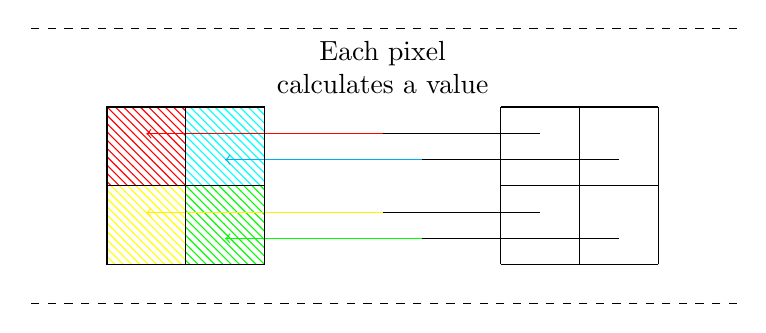
\begin{tikzpicture}[xscale=-1]
			\draw[pattern=north west lines, pattern color=green] (5, 0) rectangle (6,1);
			\draw[pattern=north west lines, pattern color=yellow] (6, 0) rectangle (7,1);
			\draw[pattern=north west lines, pattern color=cyan] (5, 1) rectangle (6,2);
			\draw[pattern=north west lines, pattern color=red] (6, 1) rectangle (7,2);
			
			\draw[step=1.0,black] (0, 0) grid (2,2);
			
			\foreach \x in {0.5,..., 1.5} {
				\foreach \y in {0,..., 1} {
					\draw[-] (\x, {\y + 0.33 * (\x + 0.5)}) -- (\x + 2.5, {\y + 0.33 * (\x + 0.5)});
				}
			}
			
			\draw [->, color=green]  (3, .33) -- (5.5, .33);
			\draw [->, color=yellow] (3.5, .66) -- (6.5, .66);
			\draw [->, color=cyan]   (3, 1.33) -- (5.5, 1.33);
			\draw [->, color=red]    (3.5, 1.66) -- (6.5, 1.66);
			
			\node[align=center] at (3.5 ,2.5) {Each pixel\\ calculates a value};
			
			\draw[step=1,black] (5, 0) grid (7, 2);
			
			\draw[dashed] (-1,-.5) -- (8, -.5);
			\draw[dashed] (-1,3) -- (8, 3);
		\end{tikzpicture} \\
		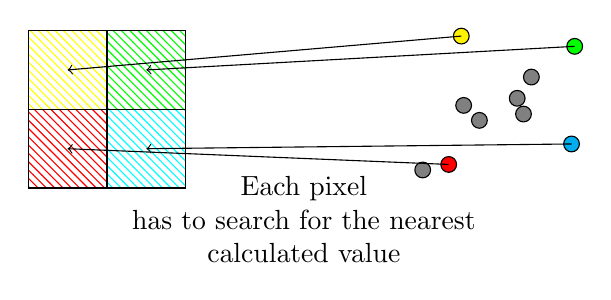
\begin{tikzpicture}[scale=-1]
		%first fill circles with gray, then draw border later
		\foreach \x in {
			{0.1, 1.44},{1.47, 0.95},{0.61, 0.59},{1.66, 1.7},{0.71, 1.06},{0.79, 0.86},{1.27, 1.14},{0.06, .2},{1.99, 1.77},{1.5, 0.07}} {
			\fill[gray] (\x) circle[radius=.1];
		}
	
		\fill[color=green] (0.06, .2)  circle[radius=.1];
		\fill[color=yellow] (1.5, 0.07) circle[radius=.1];
		\fill[color=cyan] (0.1, 1.44) circle[radius=.1];
		\fill[color=red] (1.66, 1.7) circle[radius=.1];
		
		\draw[pattern=north west lines, pattern color=green] (5, 0) rectangle (6,1);
		\draw[pattern=north west lines, pattern color=yellow] (6, 0) rectangle (7,1);
		\draw[pattern=north west lines, pattern color=cyan] (5, 1) rectangle (6,2);
		\draw[pattern=north west lines, pattern color=red] (6, 1) rectangle (7,2);
		
		%draw borders of circles after color has been drawn
		\foreach \x in {
			{0.1, 1.44},{1.47, 0.95},{0.61, 0.59},{1.66, 1.7},{0.71, 1.06},{0.79, 0.86},{1.27, 1.14},{0.06, .2},{1.99, 1.77},{1.5, 0.07}} {
			\draw (\x) circle[radius=.1];
		}
		
	
		\draw [->] (0.06, .2) -- (5.5, .5);
		\draw [->] (1.5, 0.07) -- (6.5, .5);
		\draw [->] (0.1, 1.44) -- (5.5, 1.5);
		\draw [->] (1.66, 1.7) -- (6.5, 1.5);
		
		\node[align=center] at (3.5 ,2.4) {Each pixel\\has to search for the nearest\\calculated value};
		
		\draw[step=1,black] (5, 0) grid (7, 2);
		\end{tikzpicture}
	\end{figure}

	\begin{table}[h!]
		\centering
		\label{tab:java_0_0_1}
		\caption{Changelog for Java 0.0.1}
		\begin{tabular}{p{.3 \textwidth}|p{.7 \textwidth}}
			Class name & Class description \\ 
			\hline 
			\verb|CalculationResult|&  This class stores the calculated information in an \verb|ArrayList|, which is initialized by the constructor with a given size. I have done this because each time the list has to be resized, all the elements in it have to be copied into a new array. Another feasible approach to solve the resizing problem would have been to use a \verb|LinkedList|, as they can be expanded instantly and use only as much memory as they are big, but their performance suffers greatly when accessed randomly (as opposed to sequentially). \newline
			The datatype stored in the list is defined as a generic type, and is currently the \verb|CalculationResult.DataMandelbrot| class. Furthermore, the class implements the \verb|Iterable| interface, so that it can be used in \verb|foreach| loops. \\
			\hline 
			\verb|CalculationResult.|\linebreak \hspace*{50 pt}\verb|DataMandelbrot|& This class stores one calculated point of the Mandelbrot set. The coordinates are stored as two doubles named \verb|x| and \verb|y|, the actual value is a boolean called \verb|value|, which is true for all points in the set and false for all the others.\\ 
			\hline 
			\verb|MandelbrotCalculator|& This class does the actual mathematics regarding the Mandelbrot set. The generation is started by calling the method \verb|calculate|, which then returns an instance of \verb|CalculationResult| with all the calculated points.
			Apart from that it also holds an instance of the settings, meaning that other components must access this one to get a hold on the settings, like defining the viewport. \\ 
			\hline
			\verb|FileManager|& This is the class which interacts with the filesystem. It is currently useless, because it implements a sole method, which saves an image to a file. I have only included this class, so all the code related to saving will not end up in a random class but in a specific one. This way the requirement of madularization is being fulfilled. \\ 
			\hline
			\verb|ImageCreator|& The image creator converts raw data to an image. For now, it only has to create an image from the data retrieved from the \verb|MandelbrotCalculator|. The challenge here is that the calculated points' coordinates do not match the exact coordinates of the image. Thus, each pixel has to search for the nearest point in the data set. This is a lengthy process, but I will go into more detail below. \\ 
			\hline 
			\verb|SettingsManager|& The \verb|SettingsManager| contains all preset parameters and information required to calculate the fractal. The settings are stored in a \verb|LinkedHashMap| and accessible through the methods provided. The elements of the list must implement the \verb|Setting| interface and its inherited method \verb|identifier()|. There are currently only two settings available, the \verb|SettingViewport| and the \verb|SettingNumber|, which store data for the viewport and data that can be expressed in scalars respectively. \\ 
			\hline 
			\verb|TestMain|& As the name suggests, this mainclass is only here to test the components. It replaces a proper frontend, which I have not yet created because of the big amount of work associated with it. \\ 
		\end{tabular} 
	\end{table}
	
	
	\section{Libraries}
	Used (or planned) libraries:\\
	ffmpeg for video\\
	PPM (self coded for debugging)\\
	stb for PNG (https://github.com/nothings/stb)\\
\end{document}